\chapter[]{La nascita dei fazzoletti per istruzione militare}
\graphicspath{ {./images/chapter1/} }

\begin{figure}[h]
	\centering
		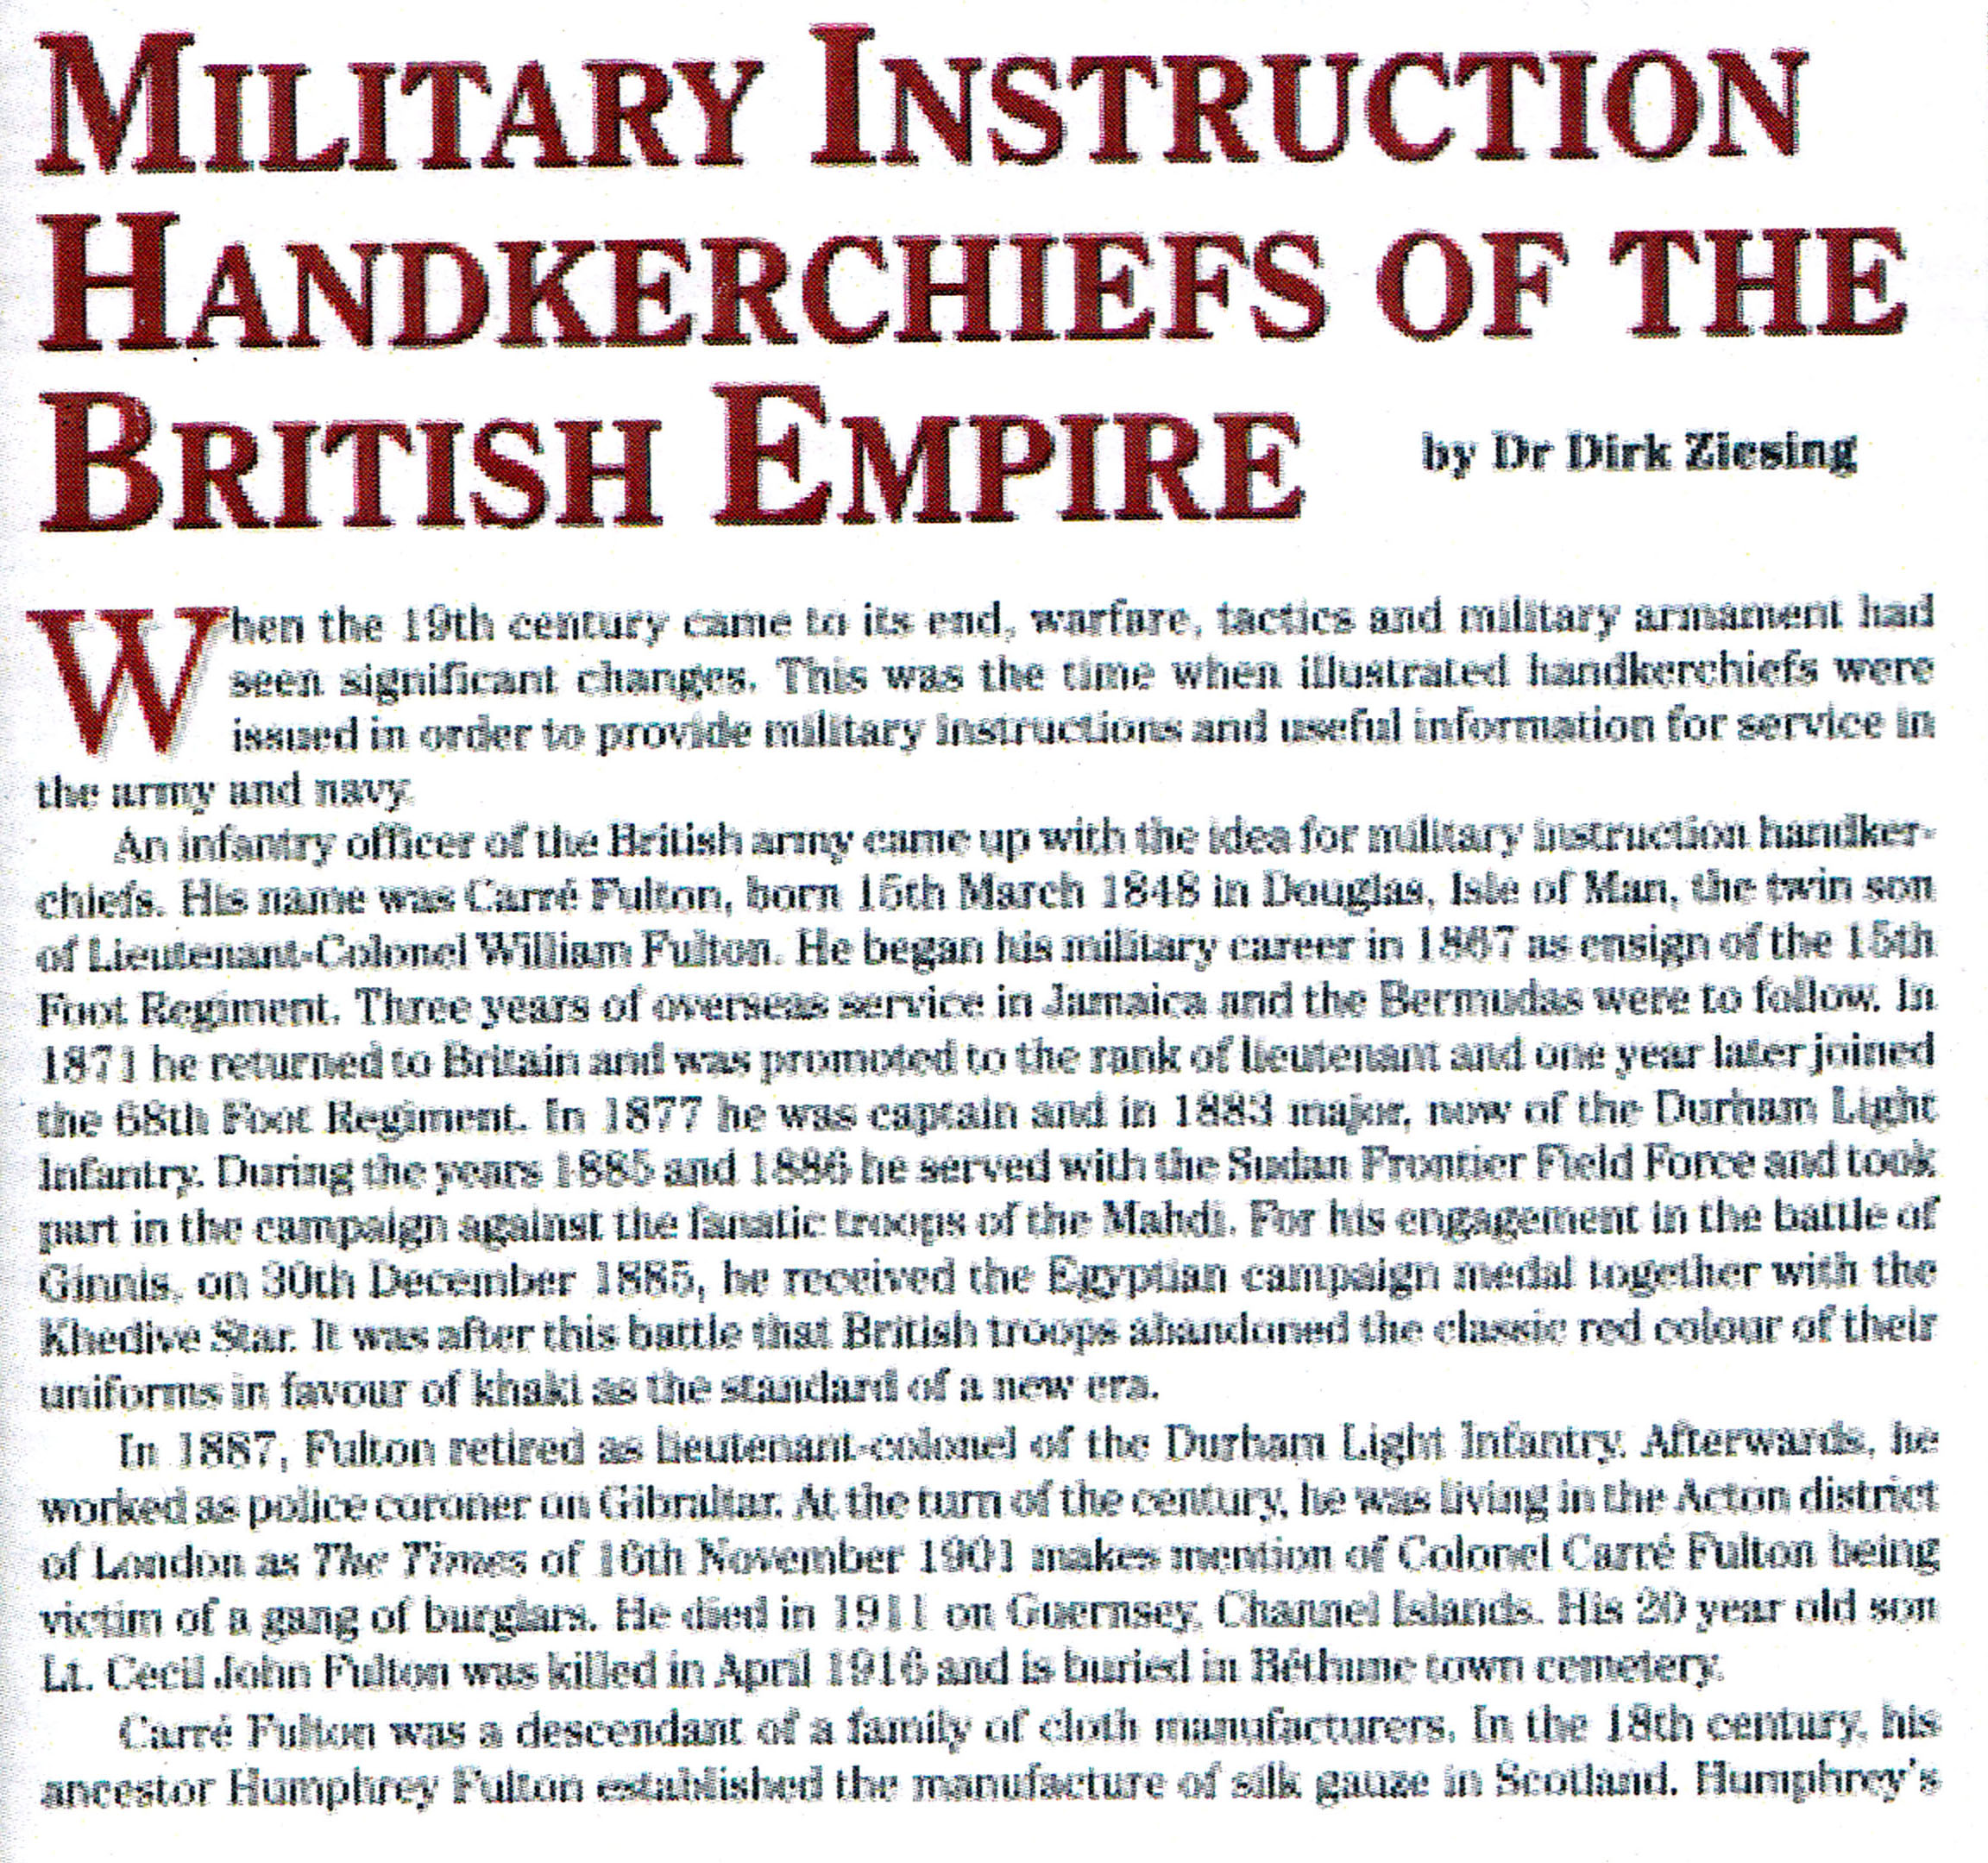
\includegraphics[width=\textwidth]{britishEmpire.jpg}
	\caption{}
	\label{fig:britishEmpire}
\end{figure}

\newpage

I FAZZOLETTI CON ISTRUZIONI MILITARI 
    DELL’IMPERO BRITANNICO

   Quando il 19° secolo arrivò alla sua fine, strategie di guerra, tattiche e armamenti militari videro significativi cambiamenti. Questo fu il periodo della creazione dei fazzoletti illustrati,  allo scopo di fornire istruzioni militari e utili informazioni per il servizio militare e navale.
   Un ufficiale della fanteria dell’esercito Britannico ebbe l’idea di queste istruzioni militari illustrate su fazzoletti. Il suo nome è Carrè Fulton, nato il 15 marzo 1848 a Douglas, nell’Isola di Man, figlio gemello del Tenente-Colonnello William Fulton. Egli iniziò la sua carriera militare nel 1867 come fante del 15° Reggimento a piedi. Seguirono 3 anni di servizio oltremare in Giamaica e nelle Bermuda. Nel 1871 egli tornò in Gran Bretagna e fu promosso al grado di tenente e un anno dopo entrò a far parte del 68° Reggimento a piedi. Nel 1877 divenne capitano e nel 1883 maggiore, questa volta della fanteria leggera di Durham. Durante gli anni 1885 e 1886 egli servì  il corpo militare di frontiera di stanza in Sudan  e prese parte alla campagna contro le truppe della resistenza anticoloniale del Mahdi. 1 (vedi nota a pag. 36).
  Per la sua partecipazione alla battaglia di Ginnis, il 30 dicembre 1885 egli ricevette la medaglia per la campagna di Egitto insieme alla stella di Khedive. 
Fu dopo questa battaglia che le truppe Britanniche abbandonarono il classico colore rosso delle loro uniformi a favore del colore cachi, quale principio di una nuova era.
   Nel 1887, Fulton si ritirò con la carica di sottotenente-colonnello della fanteria leggera di  Durham.  Successivamente egli lavorò come poliziotto a Gibilterra. Al cambio del secolo, si sa che egli viveva nel quartiere di Acton a Londra, poiché il 16 novembre 1901 il Times menzionò il colonello Carrè Fulton in quanto vittima di una banda di ladri. Egli morì nel 1911 a Guernsey, un’isola del Canale della Manica. Suo figlio ventenne, il sottotenente Cecil John Fulton fu ucciso nell’aprile del 1916 e fu seppellito nel cimitero della città di Bethune (Francia).Carrè Fulton era un discendente di una famiglia di fabbricanti di stoffa. Nel 18° secolo il suo antenato Humphrey Fulton stabilì la manifattura della garza di seta in Scozia.

\newpage
   
\begin{figure}[h]
	\centering
		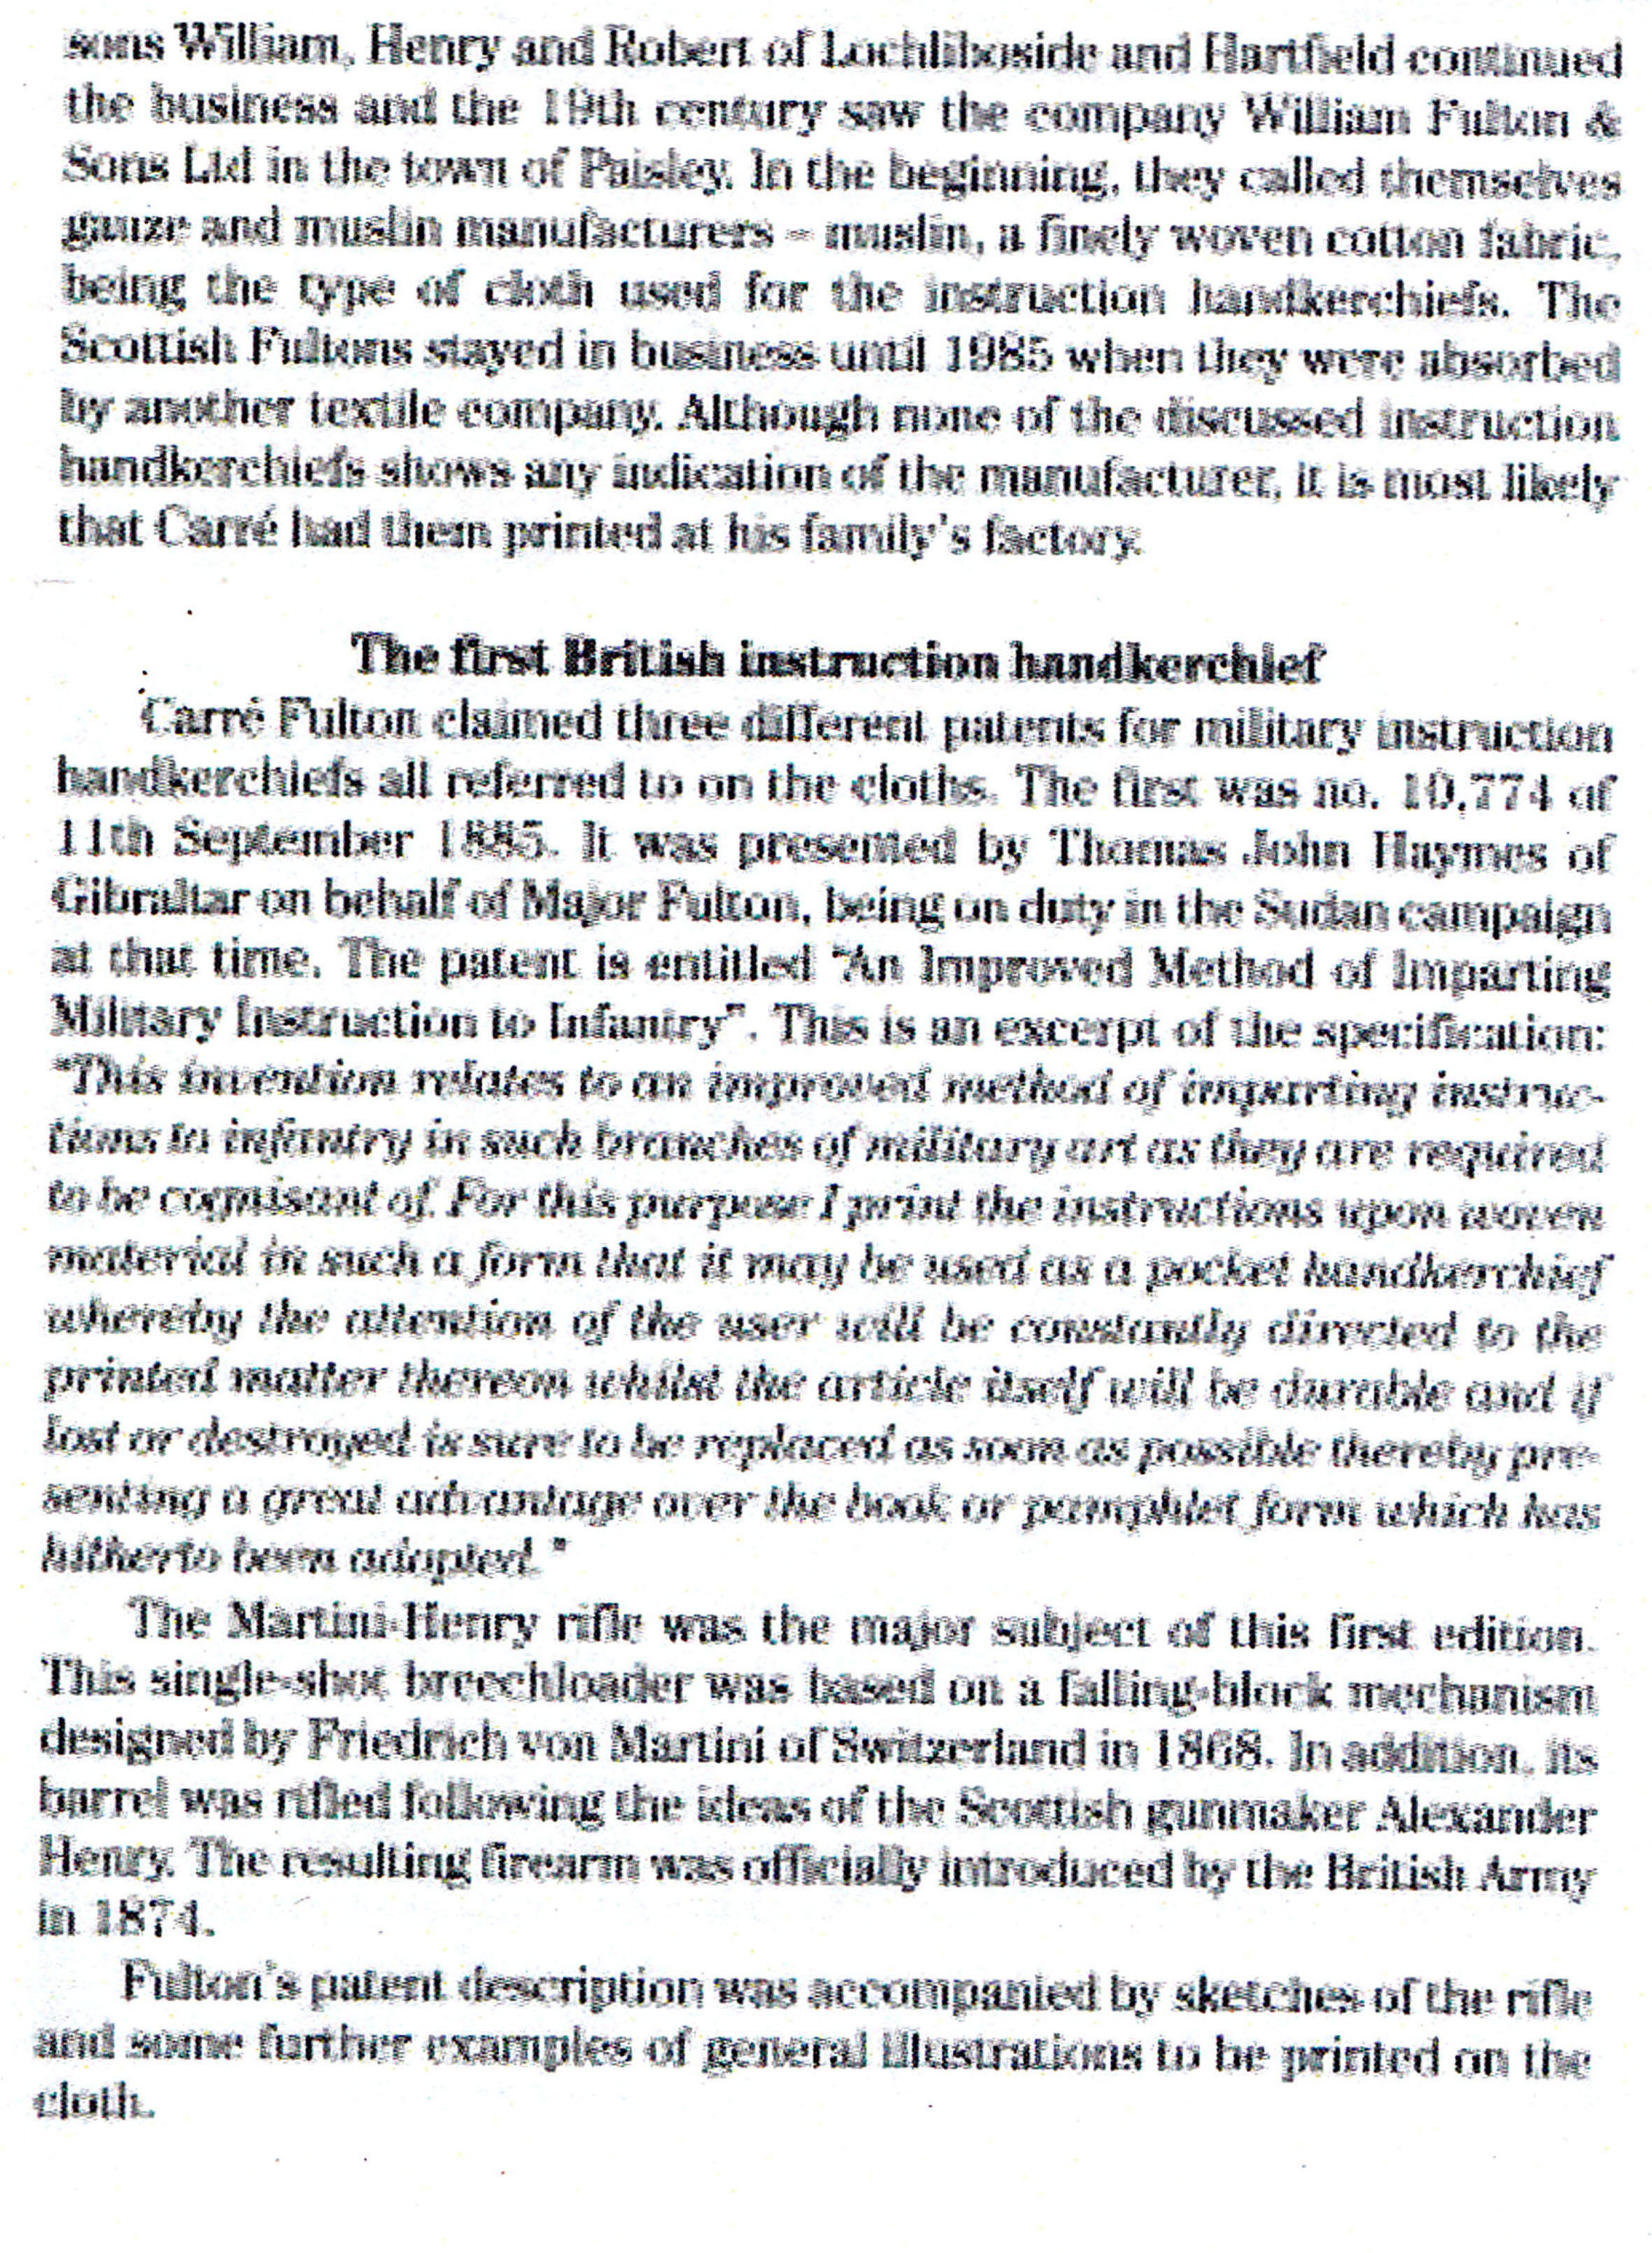
\includegraphics[width=\textwidth]{britishInstruct.jpg}
	\caption{}
	\label{fig:britishInstruct}
\end{figure}

\newpage

I figli di Humphrey, William, Henry e Robert di Lochliboside e Hartfield continuarono l’attività e il 19° secolo vide l’azienda William Fulton \& figli Ltd nella città di Paisley (Scozia). All’inizio essi si definirono produttori di garza e mussola; la mussola, un cotone intessuto finemente, divenne la stoffa  utilizzata per i fazzoletti con le istruzioni. Gli scozzesi Fulton mantennero l’attività fino al 1985 quando vennero acquisiti da un’altra società tessile. Malgrado nessuno dei citati fazzoletti con le istruzioni mostri alcuna indicazione del fabbricante, è molto probabile che Carrè li stampò nell’azienda di famiglia.

IL PRIMO FAZZOLETTO BRITANNICO CON ISTRUZIONI

   Carrè Fulton ottenne 3 diversi brevetti per le istruzioni militari sui fazzoletti, tutte stampate su stoffe. Il primo fu il n. 10.774 dell’11 settembre 1885. Questo fu presentato da Thomas John Hayrnes di Gibilterra al posto del Maggiore Fulton, impegnato nella campagna in Sudan a quel tempo. Il brevetto è intitolato “Un metodo migliore per impartire le Istruzioni Militari alla Fanteria”.  Questo un estratto della spiegazione: “ Questa invenzione si riferisce a un metodo migliore per impartire le istruzioni alla fanteria per quei rami dell’arte militare di cui devono essere a conoscenza. A questo scopo io stampo le istruzioni sopra il tessuto, in modo tale che possa essere  usato come fazzoletto tascabile. In questo modo l’attenzione dell’utilizzatore sarà costantemente diretta all’argomento stampato sino a quando l’oggetto in sé sia ancora utilizzabile e, in caso di perdita o distruzione, è sicuro che venga sostituito non appena possibile, rappresentando così un grande vantaggio rispetto al libro o l’opuscolo fin qui adottato.” 
   Il fucile Martini Henry fu il principale soggetto di questa prima edizione. Questo fucile a retro carica a colpo singolo fu basato su di un meccanismo di otturatore disegnato dallo svizzero Friedrich von Martini nel 1868. In aggiunta la sua canna fu rigata seguendo le idee del fabbricante di pistole scozzese Alexander Henry. L’arma da fuoco che ne risultò fu introdotta ufficialmente nell’esercito Britannico nel 1874.
   
\newpage

   
   
